% Template for Cogsci submission with R Markdown

% Stuff changed from original Markdown PLOS Template
\documentclass[10pt, letterpaper]{article}

\usepackage{cogsci}
\usepackage{pslatex}
\usepackage{float}
\usepackage{caption}

% amsmath package, useful for mathematical formulas
\usepackage{amsmath}

% amssymb package, useful for mathematical symbols
\usepackage{amssymb}

% hyperref package, useful for hyperlinks
\usepackage{hyperref}

% graphicx package, useful for including eps and pdf graphics
% include graphics with the command \includegraphics
\usepackage{graphicx}

% Sweave(-like)
\usepackage{fancyvrb}
\DefineVerbatimEnvironment{Sinput}{Verbatim}{fontshape=sl}
\DefineVerbatimEnvironment{Soutput}{Verbatim}{}
\DefineVerbatimEnvironment{Scode}{Verbatim}{fontshape=sl}
\newenvironment{Schunk}{}{}
\DefineVerbatimEnvironment{Code}{Verbatim}{}
\DefineVerbatimEnvironment{CodeInput}{Verbatim}{fontshape=sl}
\DefineVerbatimEnvironment{CodeOutput}{Verbatim}{}
\newenvironment{CodeChunk}{}{}

% cite package, to clean up citations in the main text. Do not remove.
\usepackage{apacite}

% KM added 1/4/18 to allow control of blind submission


\usepackage{color}

% Use doublespacing - comment out for single spacing
%\usepackage{setspace}
%\doublespacing


% % Text layout
% \topmargin 0.0cm
% \oddsidemargin 0.5cm
% \evensidemargin 0.5cm
% \textwidth 16cm
% \textheight 21cm

\title{How to Make a Proceedings Paper Submission}


\author{{\large \bf Morton Ann Gernsbacher (MAG@Macc.Wisc.Edu)} \\ Department of Psychology, 1202 W. Johnson Street \\ Madison, WI 53706 USA \AND {\large \bf Sharon J.~Derry (SDJ@Macc.Wisc.Edu)} \\ Department of Educational Psychology, 1025 W. Johnson Street \\ Madison, WI 53706 USA}


\begin{document}

\maketitle

\begin{abstract}
Include no author information in the initial submission, to facilitate
blind review. The abstract should be one paragraph, indented 1/8 inch on
both sides, in 9\textasciitilde point font with single spacing. The
heading `Abstract' should be 10\textasciitilde point, bold, centered,
with one line of space below it. This one-paragraph abstract section is
required only for standard six page proceedings papers. Following the
abstract should be a blank line, followed by the header `Keywords' and a
list of descriptive keywords separated by semicolons, all in
9\textasciitilde point font, as shown below.

\textbf{Keywords:}
Add your choice of indexing terms or keywords; kindly use a semi-colon;
between each term.
\end{abstract}

\hypertarget{introduction}{%
\section{Introduction}\label{introduction}}

Whether to keep looking at a current target of attention is one of the
most fundamental decisions we make, whether we are trying to find our
way in a busy street or swiping through TikTok. Even young infants are
tasked with making the decision on selecting what to look at and for how
long. To look or not to look, this decision that infants make constantly
has provided developmental researchers an opportunity to investigate
infants' mental world. Through the use of looking time paradigms,
researchers are able to make inferences about infants' learning and
mental representations based on changes in looking time (CITE, CITE,
CITE). In a typical experiment, infants increasingly decrease their
looking duration upon seeing repeated stimulus (i.e.~habituation). When
habituated, infants regain their interests when seeing a novel stimulus
(i.e.~dishabituation). While both phenomena are well-documented, the
factors that influence these looking time trajectories remain relatively
underexplored. A better understanding of what shapes habituation and
dishabituation is critical given their methodological and theoretical
significance. The rise and fall in looking time is not only central to
understanding infants' mental representation, but also shed light on
principles that guide information-seeking behavior in general.

Classical theory of infant looking behavior suggests three factors are
crucial to habituation and dishabituation: complexity, familiarization
time, and infants' age (Hunter \& Ames, 1988). More perceptually complex
stimuli take longer time for infants to habituate. Longer
familiarization time to one stimulus would make infants more likely to
dishabituate to another stimulus. The older infants are, the more
efficient they are at information processing, and the faster they are to
habituate when other factors are controlled for. Together, these three
factors determine how infants' looking time changes during an
experiment. Although Hunter \& Ames (1988) is influential, the evidence
for the theory is weak, with some studies showing mixed results (CITE
meta analysis). Furthermore, this verbal theory lacks quantitative
details, and therefore unlikely to offer precise predictions on looking
time changes based on the different factors.

In contrast to verbal theory, computational models offer quantitative
predictions. More recent work has linked infants' looking behaviors with
a range of information theoretic measurements derived from models. In
pioneering work, KPA (CITE) developed a paradigm in which infants are
shown sequences of events. Infants' look-away probabilities toward the
stimuli are compared with surprisal, a measure of information content,
derived from a rational learner model that keeps track of the
probabilities of each event. The study shows that infants looking
behaviors can be predicted by surprisal. In particular, they pay most
attention to event sequences that are neither too high nor too low in
surprisal. A recent study with a similar paradigm provides an
alternative linking hypothesis. In Poli et al (2020), another
information theoretic measurement, Kullback-Leibler divergence, is shown
to outperform surprisal in predicting infants' looking time. These
attempts on connecting information theoretic measurements to infants'
looking time resonate with the emerging literature on curiosity in
developmental robotics and reinforcement learning (CITE, CITE, CITE).
Curiosity-driven artificial agents' exploratory behaviors are guided by
optimizing Expected Information Gain (EIG) (CITE, CITE), a measurement
that has been shown to be related to information-seeking in human
children and adults as well (CITE).

However, there are several limitations to the existing models. First,
the current models did not capture the noisy nature of perceptual
learning (CITE noisy perception?). The rational learner models were
assumed to acquire perfect representation of each event in the sequence
(CITE model). This assumption leads to the second limitation: the lack
of explanation in why a learner would choose to learn a stimulus in the
first place. Both surprisal and KL-divergence have been presented as
potential explanations of infants' looking behaviors, yet neither of the
measurements is mechanistically linked to the models' behaviors. They
are descriptive in nature, derived from models that track the
probabilities of the events. Finally, the behavioral data that the
models were evaluated with came from experimental paradigms that were
not representatives of infant looking time paradigms. The key phenomena,
habituation and dishabituation, were not captured. The extent to which
we can extrapolate current behavior-model fits to understand changes in
looking time in a typical looking time experiment remains limited.

Here we present a series of models that can explain patterns in looking
time. Our Goal is to provide a unifying quantitative account of looking
behaviors as arising from optimal decision-making over noisy perceptual
representations (CITE C \& G; drif diffusion). We begin by instantiating
a version of prior learning models in an independent-trial format (where
individual stimuli are learned, not sequences of events). We then
develop a second model that addresses weakness in previous work by a)
assume the model is accumulating noisy samples from the stimulus, and b)
assume the model is choosing what to look at depending on the linking
hypotheses (surprisal, KL-divergence, and EIG). FInally, we evaluate our
model with adult looking time data collected from a paradigm that
captures habituation, dishabituation, and complexity effect.

\hypertarget{models}{%
\section{Models}\label{models}}

\#\texttt{\{r\ child\ =\ "02\_model.Rmd"\}\ \#}

\hypertarget{experiment}{%
\section{Experiment}\label{experiment}}

\hypertarget{methods}{%
\subsection{Methods}\label{methods}}

\hypertarget{participants}{%
\subsubsection{Participants}\label{participants}}

We recruited 449 participants (Age \emph{M} = 30.83; \emph{SD} = 17.44)
on Prolific. They were randomly assigned to one of the three conditions
of the experiment (Curiosity: \emph{N} = 156; Memory: \emph{N} = 137;
Math: \emph{N} = 156). Participants were excluded if they showed
irregular reaction times or their responses in the filler tasks
indicates low engagement with the experiment. All exclusion criteria
were pre-registered. The final sample included N participants (Curiosity
\emph{N} = 143; Memory: \emph{N} = 98; Math: N = \emph{N} = 139).

\hypertarget{procedure}{%
\subsubsection{Procedure}\label{procedure}}

This is a web-based self-paced visual presentation task. Participants
were instructed to look at a sequence of animated creatures at their own
pace and answer some questions throughout. At the end of the experiment,
participants were asked to rate the similarity between pairs of
creatures and complexity of creatures they encountered on a 7-point
Likert Scale. Each participant saw eight blocks in total, half of which
used creatures with high perceptual complexity, and half of which used
creatures with low perceptual complexity. On each trial, an animated
creature showed up on the screen. participants can press the down arrow
to go to the next trial whenever they want after a minimum viewing time
of 500 ms.

Each block consisted of six trials. A trial can be either a background
trial (B) or a deviant trial (D). A background trial presented a
creature repeatedly, and the deviant trial presented a different
creature from the background trial in the block. Two creatures in the
blocks were matched for visual complexity. There were four sequences of
background trials and deviant trials. Each sequence appeared twice, once
with high complexity stimuli and once with low complexity stimuli. The
deviant trial can appear at either the second (BDBBBB), the fourth
(BBBDBB), or the sixth trial (BBBBBD) in the block. Two blocks do not
have deviant trials (BBBBBB). The creatures presented in the deviant
trials and background trials were matched for complexity.

Participants were randomly assigned to one of the three conditions:
Curiosity, Memory, and Math The three conditions only differed in the
type of questions asked following each block. In Curiosity condition,
participants were asked to rate ``How curious are you about the
creature?'' on a 5-point Likert scale. In Memory condition, a
forced-choice recognition question followed each block (``Have you seen
this creature before?''). The creature used in the question in both
conditions was either a creature presented in the preceding block or a
novel creature matched in complexity. In Math condition, the
participants were asked a simple arithmetic question (``What is 5 +
7?'') in multiple-choice format.

\hypertarget{stimuli}{%
\subsubsection{Stimuli}\label{stimuli}}

The animated creatures (Fig 1) were created using Spore (a game
developed by Maxis in 2008). There were forty creatures in total, half
of which have low perceptual complexity (e.g.~the creatures do not have
limbs, additional body parts, facial features, or textured skin), and
half of which have high perceptual complexity (i.e.~they do have the
aforementioned features). We used the ``animated avatar'' function in
Spore to capture the creatures in motion.

\hypertarget{results}{%
\subsection{Results}\label{results}}

\hypertarget{analytic-approach}{%
\subsubsection{Analytic Approach}\label{analytic-approach}}

The sample size, methods, and main analyses were all pre-registered and
are available at {[}LINK{]}. Data and analysis scripts are available at
{[}LINK{]}.

\hypertarget{manipulation-check}{%
\subsubsection{Manipulation Check}\label{manipulation-check}}

The complex animated creatures were rated as more perceptually complex
(M = ; SD = ) than the simple animated creatures (M = ; SD = ). Pairs of
background creature and deviant creature were rated as moderately
dissimilar to one another (M = ; SD = ).

\hypertarget{evaluating-the-paradigm}{%
\subsubsection{Evaluating the Paradigm}\label{evaluating-the-paradigm}}

\begin{CodeChunk}
\begin{CodeOutput}
Linear mixed model fit by REML. t-tests use Satterthwaite's method [
lmerModLmerTest]
Formula: log(trial_looking_time) ~ I(exp(1)^(-trial_number)) * trial_type *  
    block_type + (1 | subject)
   Data: d

REML criterion at convergence: 37415.2

Scaled residuals: 
    Min      1Q  Median      3Q     Max 
-3.7455 -0.6692 -0.0499  0.5968  5.4843 

Random effects:
 Groups   Name        Variance Std.Dev.
 subject  (Intercept) 0.2752   0.5246  
 Residual             0.4250   0.6519  
Number of obs: 18198, groups:  subject, 380

Fixed effects:
                                                                          Estimate
(Intercept)                                                              7.531e+00
I(exp(1)^(-trial_number))                                                2.125e+00
trial_typedeviant                                                        6.252e-01
block_typesimple_dissimilar                                             -5.175e-02
I(exp(1)^(-trial_number)):trial_typedeviant                             -2.226e+00
I(exp(1)^(-trial_number)):block_typesimple_dissimilar                   -4.028e-01
trial_typedeviant:block_typesimple_dissimilar                           -1.899e-01
I(exp(1)^(-trial_number)):trial_typedeviant:block_typesimple_dissimilar  5.833e-01
                                                                        Std. Error
(Intercept)                                                              2.843e-02
I(exp(1)^(-trial_number))                                                5.415e-02
trial_typedeviant                                                        2.737e-02
block_typesimple_dissimilar                                              1.299e-02
I(exp(1)^(-trial_number)):trial_typedeviant                              3.310e-01
I(exp(1)^(-trial_number)):block_typesimple_dissimilar                    7.652e-02
trial_typedeviant:block_typesimple_dissimilar                            3.865e-02
I(exp(1)^(-trial_number)):trial_typedeviant:block_typesimple_dissimilar  4.679e-01
                                                                                df
(Intercept)                                                              4.432e+02
I(exp(1)^(-trial_number))                                                1.781e+04
trial_typedeviant                                                        1.781e+04
block_typesimple_dissimilar                                              1.781e+04
I(exp(1)^(-trial_number)):trial_typedeviant                              1.781e+04
I(exp(1)^(-trial_number)):block_typesimple_dissimilar                    1.781e+04
trial_typedeviant:block_typesimple_dissimilar                            1.781e+04
I(exp(1)^(-trial_number)):trial_typedeviant:block_typesimple_dissimilar  1.781e+04
                                                                        t value
(Intercept)                                                             264.857
I(exp(1)^(-trial_number))                                                39.240
trial_typedeviant                                                        22.848
block_typesimple_dissimilar                                              -3.984
I(exp(1)^(-trial_number)):trial_typedeviant                              -6.724
I(exp(1)^(-trial_number)):block_typesimple_dissimilar                    -5.264
trial_typedeviant:block_typesimple_dissimilar                            -4.914
I(exp(1)^(-trial_number)):trial_typedeviant:block_typesimple_dissimilar   1.247
                                                                        Pr(>|t|)
(Intercept)                                                              < 2e-16
I(exp(1)^(-trial_number))                                                < 2e-16
trial_typedeviant                                                        < 2e-16
block_typesimple_dissimilar                                             6.82e-05
I(exp(1)^(-trial_number)):trial_typedeviant                             1.82e-11
I(exp(1)^(-trial_number)):block_typesimple_dissimilar                   1.42e-07
trial_typedeviant:block_typesimple_dissimilar                           9.01e-07
I(exp(1)^(-trial_number)):trial_typedeviant:block_typesimple_dissimilar    0.212
                                                                           
(Intercept)                                                             ***
I(exp(1)^(-trial_number))                                               ***
trial_typedeviant                                                       ***
block_typesimple_dissimilar                                             ***
I(exp(1)^(-trial_number)):trial_typedeviant                             ***
I(exp(1)^(-trial_number)):block_typesimple_dissimilar                   ***
trial_typedeviant:block_typesimple_dissimilar                           ***
I(exp(1)^(-trial_number)):trial_typedeviant:block_typesimple_dissimilar    
---
Signif. codes:  0 '***' 0.001 '**' 0.01 '*' 0.05 '.' 0.1 ' ' 1

Correlation of Fixed Effects:
               (Intr) I(x(1)^(-_)) trl_ty blck__ I(x(1)^(-_)):_ I((1)^(-_)):__
I(x(1)^(-_))   -0.196                                                         
trl_typdvnt    -0.108  0.203                                                  
blck_typsm_    -0.228  0.428        0.237                                     
I(x(1)^(-_)):_  0.032 -0.164       -0.647 -0.070                              
I((1)^(-_)):__  0.138 -0.708       -0.144 -0.606  0.116                       
trl_typd:__     0.077 -0.144       -0.708 -0.336  0.458          0.204        
I((1)^(-_)):_: -0.023  0.116        0.458  0.099 -0.708         -0.164        
               tr_:__
I(x(1)^(-_))         
trl_typdvnt          
blck_typsm_          
I(x(1)^(-_)):_       
I((1)^(-_)):__       
trl_typd:__          
I((1)^(-_)):_: -0.647
\end{CodeOutput}
\end{CodeChunk}

Three criteria were selected to evaluate whether the paradigms
successfully captured the characteristic looking time patterns observed
in infant literature: habituation (the decrease in looking time for a
stimulus with repeated presentations), dishabituation (the increase in
looking time to a new stimulus after habituated to one stimulus), and
complexity effect (longer looking time for perceptually more complex
stimuli). To evaluate the phenomenon quantitatively, we ran a linear
mixed effects model with maximal random effect structure. {[}DESCRIBE
THE MODEL{]}. {[}REPORT THE MODEL RESULTS{]}

\hypertarget{order-effect}{%
\subsubsection{Order Effect}\label{order-effect}}

\begin{CodeChunk}

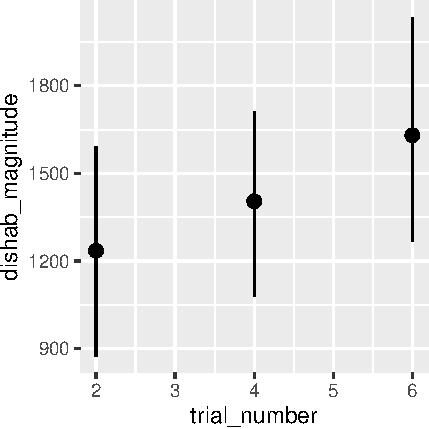
\includegraphics{figs/unnamed-chunk-9-1} \begin{CodeOutput}
Linear mixed model fit by REML. t-tests use Satterthwaite's method [
lmerModLmerTest]
Formula: dishab_magnitude ~ trial_number + (1 | subject)
   Data: dishab_d

REML criterion at convergence: 44965.3

Scaled residuals: 
    Min      1Q  Median      3Q     Max 
-7.5761 -0.3319 -0.0903  0.2873  7.5993 

Random effects:
 Groups   Name        Variance Std.Dev.
 subject  (Intercept)  2450681 1565    
 Residual             21340805 4620    
Number of obs: 2272, groups:  subject, 380

Fixed effects:
             Estimate Std. Error      df t value Pr(>|t|)    
(Intercept)   1029.26     268.80 2225.33   3.829 0.000132 ***
trial_number    99.05      59.39 1890.38   1.668 0.095529 .  
---
Signif. codes:  0 '***' 0.001 '**' 0.01 '*' 0.05 '.' 0.1 ' ' 1

Correlation of Fixed Effects:
            (Intr)
trial_numbr -0.884
\end{CodeOutput}
\end{CodeChunk}

While visualizing the data, we unexpectedly found that the position in
which the deviant trial appeared in the sequence had an effect on the
shape of the habituation and dishabituation curves. To explore this
phenomenon quantitatively, we operationalized the magnitude of
dishabituation as the difference between the looking time at the deviant
trial minus the background trial at the same position. Then, we fit a
mixed effect model with the position of deviant as fixed effect and
{[}???{]} as a random effect. We found that the position was a
significant predictor of the magnitude of dishabituation (looking time
at the deviant trial minus the background trial at the same position).
Deviant trials that appeared last elicited the strongest dishabituation
effect (M = ; SD:, ), followed by the deviant trials appeared fourth (M,
SD), with the deviant trial on the second showing the smallest amount of
dishabituation (M, SD).

\hypertarget{discussion}{%
\subsection{Discussion}\label{discussion}}

\hypertarget{general-discussion}{%
\section{General Discussion}\label{general-discussion}}

\hypertarget{references}{%
\section{References}\label{references}}

\hypertarget{references-1}{%
\section{References}\label{references-1}}

\setlength{\parindent}{-0.1in} 
\setlength{\leftskip}{0.125in}

\noindent

\bibliographystyle{apacite}


\end{document}
